\documentclass[12pt]{report}
\usepackage{amsmath}
\usepackage{amsfonts}
\usepackage{listings}
\usepackage{blindtext}
%\usepackage{biblatex}
\usepackage[colorlinks=true]{hyperref}
\usepackage{enumitem}
\usepackage{mathtools}
\usepackage{graphics}
\usepackage{graphicx}
\usepackage{float}
\usepackage{cancel}
\usepackage[margin=1in]{geometry}
\usepackage{tikz}
%\addbibresource{references.bib}

\usetikzlibrary{automata, positioning, arrows}
\usetikzlibrary{matrix,chains,positioning,decorations.pathreplacing,arrows}
\title{
Conventional Neuroevolution for Handwritten Digit Classification% Make sure you change this
}
\author{Nathan Smith \\\footnotesize
Student number: 20105878\\}
\date{
December 12, 2021% Make sure you change this
}
\begin{document}

\begin{titlepage}
    \maketitle
\end{titlepage}

\section*{Problem Description}
The brain is one of the most complex devices known to us as humans at this point in time
allowing us to do all the things we've accomplished today. We've attempted to mimic
the power of the brain through the use of neural networks, a simple approximation of
how we think, allowing the computers we've built to do the same. In this project, we
take a look at the training of such a network to see if a more successful approach to learning
can be found, as opposed to the typical implementation of stochastic gradient descent. I
decided to take on the task of implementing conventional neuroevolution to the network
to see how well it performs overall.

\par This project is the implementation of an evolutionary algorithm applied to neural
networks of fixed topology, in order to train their weight and bias values to categorize
an image set of handwritten digits. 
The fixed topology or 'conventional' design was selected not only due to ease of 
implementation, but also to allow for a more fair comparison of the neuroevolutionary
approach against backpropagation as both networks are of the same structure, and only their
weight and bias values differ. The main idea for this project was to compare an
evolutionary exploration approach for neural network training to the
more popular method of backpropagation and gradient descent.


\section*{EA Design}
The evolutionary algorithm has a population of neural network objects, each containing their
respective weight and bias values. We'll discuss how each main section of the evolutionary
algorithm was implemented and the design choices behind why we did it.


\subsection*{Main evolutionary algorithm}

\subsubsection*{Population initialization}
Population initialization is quite simple thanks to the implementation of a neural network object we
created. This is simply a matter of appending to the total population list a
new neural network object initialized with random values about a mean of 0. The only value we
use to initialize the neural network object is a structure tuple, which dictates
the structure the neural network will take on - it's important all entities within
the population are identical in this respect.

\subsubsection*{Selection/Replacement}
Due to the computational power required to find essentially random
values that allow the network to function better, it's important that we
maintain genetic diversity as we continue. With this in mind, we use a tournament to select the two parents and use them to produce two
offspring, this occurs repeatedly until the entire
pool is replaced - except for two. This removes all networks that performed poorly, while essentially doing
a search in the direction that seems most likely to bear better networks. The two most fit individuals of 
the current population make it onto the next generation as well, ensuring 
there is always an optimal candidate within the population and to ensure we don't devolve.  
 
\subsubsection*{Crossover}
There are two main methods for crossover that were used within this project.
The first is where each child starts off as an exact copy of each parent. We then iterate through each
weight value of each child and have some chance to swap their values. The other method used
is akin to one point crossover, except applied to each layer of neurons separately. We 
iterate through each layer, and randomly swap entire neurons beyond a specific random
point between the children. For example, using the diagram below, this one point crossover
would first choose a random value between 0 and 3, and swaps each neuron in the hidden layer
between the two children, along with all their weights; it then moves on to the next layer, and
does this repeatedly until it reaches the end.

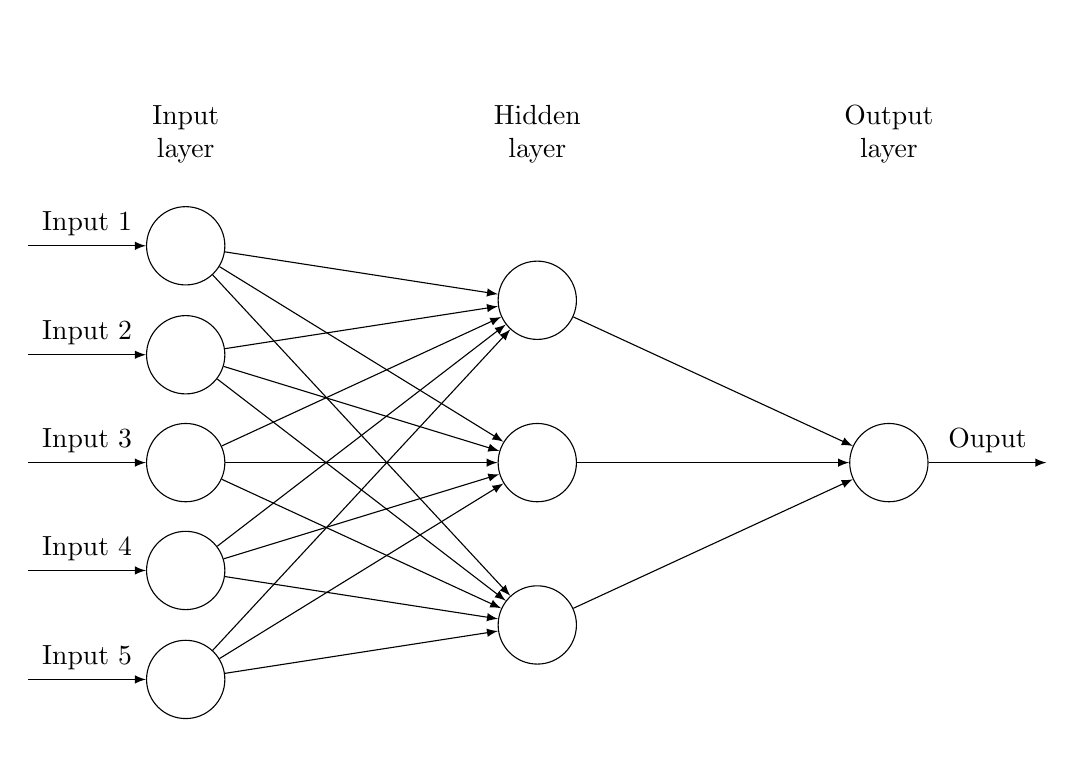
\begin{tikzpicture}[
    plain/.style={
        draw=none,
        fill=none,
        },
    net/.style={
        matrix of nodes,
        nodes={
        draw,
        circle,
        inner sep=10pt
        },
        nodes in empty cells,
        column sep=2cm,
        row sep=-9pt
        },
    >=latex
    ]
    \matrix[net] (mat)
    {
    |[plain]| \parbox{1.3cm}{\centering Input\\layer} & |[plain]| \parbox{1.3cm}{\centering Hidden\\layer} & |[plain]| \parbox{1.3cm}{\centering Output\\layer} \\
    & |[plain]| \\
    |[plain]| & \\
    & |[plain]| \\
        |[plain]| & |[plain]| \\
    & & \\
        |[plain]| & |[plain]| \\
    & |[plain]| \\
        |[plain]| & \\
    & |[plain]| \\    };
    \foreach \ai [count=\mi ]in {2,4,...,10}
        \draw[<-] (mat-\ai-1) -- node[above] {Input \mi} +(-2cm,0);
    \foreach \ai in {2,4,...,10}
    {\foreach \aii in {3,6,9}
        \draw[->] (mat-\ai-1) -- (mat-\aii-2);
    }
    \foreach \ai in {3,6,9}
        \draw[->] (mat-\ai-2) -- (mat-6-3);
    \draw[->] (mat-6-3) -- node[above] {Ouput} +(2cm,0);
\end{tikzpicture}


\subsubsection*{Mutation}
This function was applied directly within the neural network object as opposed to
within the main evolutionary program because mutation was easier as a property of
the network, allowing it to manipulate its own weights. How we go about
mutation is similar to crossover; we iterate over every
weight and bias value, and with an equally random chance we do one of four
mutations: replace whatever value is there with a newly generated one, effectively 
resetting it; we multiply the weight value by some random value distributed around 1;
we add/subtract a small value from the weight, or lastly, we change the sign of the
weight. One of these four mutations occur with a random chance on a random
amount of weights, dictated by the mutation chance parameter. 
\par This method was implemented due to it being the most ideal for this situation.
Originally, only replacement was implemented, however in order to nudge more sensitive
networks later on in the training process, resetting weights provided too much of a
shift, so manipulations were added to allow nudging to be done, instead of a
pure random approach to weight mutation. 
\par Due to the way this method was implemented it's by far the most computationally
taxing part of the program, with its computational cost being directly proportional
to the mutation rate. A lower mutation means a faster execution time due to fewer
weights being changed, and consequently, heavy mutation results in large time increase
per loop. 
\par Lastly, we implemented a decay rate to the mutation rate. This allows for more
mutation to occur at the start of the program and taper off at larger epochs. This
was done because a constant mutation rate made tweaking the network at later epochs
much more volatile than at the beginning. To find better weight values for the network,
making mutations at the same rate as at the beginning of the program reduces our chance
to find an improvement, since such dramatic changes are being made. The decaying mutation
allows for less and less exploration of weight values once we get a better network base.
The decaying mutation rate also helps to speed up the simulation as time progresses.


\subsubsection*{Fitness}
The implementation of this within the program is combined with evaluation into one function.
It was unnecessary to split evaluation and fitness into two separate functions, especially
considering fitness relies on the results on a per-image basis - it would be costly
to go back through each image to calculate the fitness after evaluation; hence they are
done in the same loop.

\par The fitness used is that of the cost for the backpropagation approach, that being the
sum of the squared errors. Using the accuracy of each neural network would be the most
obvious choice, however utilizing the cost allows for networks overall closer to the
actual values to succeed more. Using cost as opposed to accuracy lends us additionally
the ability to more easily compare this neuroevolution approach to backpropagation.
Calculating the cost function is simply taking the sum of the squared differences
between the network output and the desired output, an example of this is provided below.
Where $\vec{i}$ contains the values the network predicts, and $\vec{x}$ is the
vector containing the correct digit.
\begin{equation*}
    C(\vec{i}) = 
    \begin{cases}
        (i_0-x_0)^2+& \\
        (i_1-x_1)^2+& \\
        (i_2-x_2)^2+& \\
        (i_3-x_3)^2+& \\
        (i_4-x_4)^2+& \\
        (i_5-x_5)^2+& \\
        (i_6-x_6)^2+& \\
        (i_7-x_7)^2+& \\
        (i_8-x_8)^2+& \\
        (i_9-x_9)^2&
    \end{cases}
    \text{Example case}
    \to \begin{cases}
        (0.8-0)^2+& \\
        (0.2-0)^2+& \\
        (0.9-0)^2+& \\
        (0.1-0)^2+& \\
        (0.1-0)^2+& \\
        (0.7-1)^2+& \\
        (0.3-0)^2+& \\
        (0.2-0)^2+& \\
        (0.9-0)^2+& \\
        (0.6-0)^2&
    \end{cases}
     = 2.9
\end{equation*}

When evaluating the network, we do basic matrix multiplication using the weights with
the previous layers values added with the biases. This is then passed through an activation function, in this
case ReLU, before repeating the process over again. On the final layer, we pass it
through softmax instead of ReLU to get fairly distributed choice amongst the outputs. A simple diagram of this process can be seen below.

\begin{figure}[H]
    \centering
    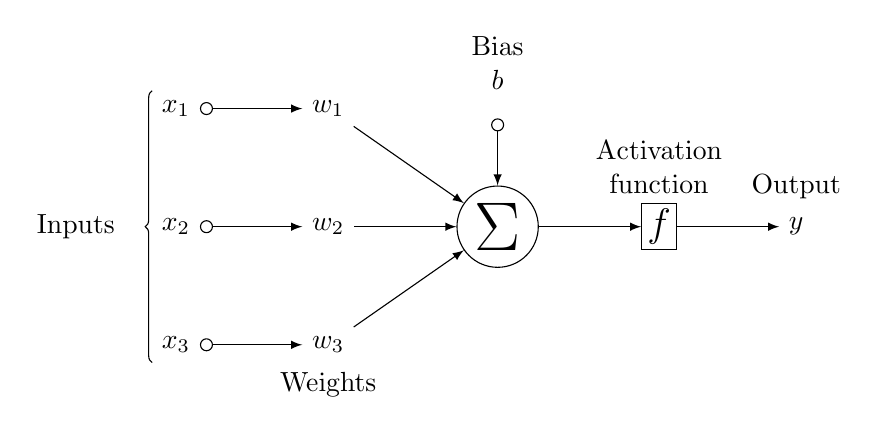
\begin{tikzpicture}[
        init/.style={
            draw,
            circle,
            inner sep=2pt,
            font=\Huge,
            join = by -latex
        },
        squa/.style={
            draw,
            inner sep=2pt,
            font=\Large,
            join = by -latex
        },
        start chain=2,node distance=13mm
        ]
        \node[on chain=2] 
            (x2) {$x_2$};
        \node[on chain=2,join=by o-latex] 
            {$w_2$};
        \node[on chain=2,init] (sigma) 
            {$\displaystyle\Sigma$};
        \node[on chain=2,squa,label=above:{\parbox{2cm}{\centering Activation \\ function}}]   
            {$f$};
        \node[on chain=2,label=above:Output,join=by -latex] 
            {$y$};
        \begin{scope}[start chain=1]
        \node[on chain=1] at (0,1.5cm) 
            (x1) {$x_1$};
        \node[on chain=1,join=by o-latex] 
            (w1) {$w_1$};
        \end{scope}
        \begin{scope}[start chain=3]
        \node[on chain=3] at (0,-1.5cm) 
            (x3) {$x_3$};
        \node[on chain=3,label=below:Weights,join=by o-latex] 
            (w3) {$w_3$};
        \end{scope}
        \node[label=above:\parbox{2cm}{\centering Bias \\ $b$}] at (sigma|-w1) (b) {};

        \draw[-latex] (w1) -- (sigma);
        \draw[-latex] (w3) -- (sigma);
        \draw[o-latex] (b) -- (sigma);

        \draw[decorate,decoration={brace,mirror}] (x1.north west) -- node[left=10pt] {Inputs} (x3.south west);
    \end{tikzpicture}
    \caption{The overall process of what goes on in the neural network}
\end{figure}

\par The time cost of evaluating the network is high - with time growing linearly
with the amount of images to evaluate. The training set we use has over 50k images,
however, only about 100 are used for training mainly due to the limiting factor of Python being too slow
to evaluate through that many images.
Using more provides little benefit and increases computation times.

\par Before evaluation can occur, we normalize the data by dividing each pixel value by
255, turning it into a number from 0 to 1. This reduces high pixel values from biasing
the network, and allows all data to be treated fairly.



\section*{EA Results}
Despite being essentially a pure random search,
it produced somewhat surprising results. The absolute highest accuracy I was able to achieve
within 1000 epochs of training was about 81\%. It should be noted all data was used
on the same set of data it was trained with, no test sets were used, so the results
may not apply well to more diverse settings and overfitting may be present.

These are the accuracy results of one of the first implementations of the algorithm. 
This used a constant mutation rate, with no crossover or breeding, only
mutation. As you can see, the results peak at about 45\% accuracy after 1000 epochs.
Since mutation is by far the most computational heavy task, this wasn't much faster than
later implementations, taking about an hour and a half to train.


Upon implementing crossover we see an increase in performance.
The parent selection for this was based on selecting the parents at the start of the
epoch and producing the children thereafter. A respectable performance gain from the
above trial.


This was when it broke through 70\% accuracy. A large milestone. This was thanks to
the decaying mutation rate, allowing for more fine-tuning of weight and bias values
as the simulation continued.

This was the best performance achieved. After implementing unique parents per child
to replace each member of the population based on a tournament; not based on a per-epoch,
but a per child method. Including all the above changes in
the previous graphs above we produced a
neuroevolutionary algorithm that was able to achieve a maximum of 81\% accuracy in about
an hour and half of training time. For completion's sake, cost is included within
the graph as well
alongside accuracy - and as you can see, they are essentially identical. 
\newline


These graphs are related to the above in that they are from the same simulation.
The graph on the left shows the time in seconds it took to calculate each epoch. As
you can see, the first roughly 100 epochs are by far the most computationally taxing due
to the high initial mutation rate. Once the mutation rate decays, the performance
stops decreasing - staying consistent at just under 6 seconds per epoch.
\par For the other graph, it details the amount of genes that are identical between
two parents when they mate. It showcases the lack of genetic diversity per epoch.
Again, for the first roughly 100 epochs when the mutation rate is high we have 
high genetic diversity, however when the mutation rate subsides we stop mutating as
much and are left with similar individuals within the population. This is by design,
as the further we make it into the simulation, the less dramatic changes we wish 
to make.

\section*{Comparison}
A comparison between a highly optimized library and a crude implementation of neuroevolution
is a bit of an unfair comparison, so to make this comparison slightly more fair, we
are going to compare it to a fairly bare-bones raw python implementation of
backpropagation taken from \cite{hansen_2020}. With this we can more accurately compare the two
algorithms. All these graphs are from using a similar dataset size
to the evolutionary algorithm.


The two graphs are of the same data point, that being the accuracy of the network
per epoch. As you can see, it varies, however it is consistently bad, which is
a surprising discovery, as the evolutionary algorithm beats in it in terms of accuracy
when using the same amount of data, and epoch count.


However, with that said, the backpropagation algorithm crushes the neuroevolutionary
approach in terms of speed. As can be seen from the graph above, to evaluate
1000 epochs takes only about 150 seconds, or 2 and a half minutes total. This
is a massive time save in comparison to the neuroevolutionary algorithm at
about 2 hours total.

\par However, all these values were with the same reduced dataset size that
the evolutionary algorithm used, which may be unfair, as the evolutionary algorithm
needs to evaluate upwards of 50 networks, whereas this algorithm need only do one.
Increasing the dataset count the algorithm uses to the full 60k,
we obtain values such as these:


Only 50 epochs were evaluated due to time, however it can be seen comparably, that
backpropagation takes the lead in terms of performance, but it lags behind in total time by a lot.
Backpropagation additionally has the strength in its consistency
in learning. If the above tests were to run for longer,
backprop would most likely outperform neuroevolution after a certain point, as 
gradient descent would be more optimal than random mutations. The reason this was not
done was mainly due to time needed to accomplish this. To evaluate a full 1000 epoch
backpropagation with these times, it would take about 12 hours to train - compared to
the 2 and a half for neuroevolution.
\par Overall, when working with a small dataset, backprop is worse in accuracy, but
significantly faster at evaluation. Conversely, with a large dataset backprop
achieves a better accuracy, at the cost of taking more time. 
\par Initially when creating this project
I thought backprop would be better overall consistently, however that does not appear
to be the case, and both algorithms have specific strengths and weaknesses when
compared to one another. 

\section*{Discussion}
So the question remains, what can be done from here?
This was a very introductory approach, and many changes could be made
to enhance it. The program was able to get around 81\% accuracy through what was
essentially random changes progressively being made. A strictly random
approach as was done here is just not the best for this type of task of tweaking
over 70k weights.
\par It was interesting to see how the neuroevolutionary approach compared to
the backpropagation approach, noting how the evolutionary algorithm achieved
its results significantly faster than backpropagation, and with small datasets,
performing better in terms of accuracy.
\par Increasing the overall complexity of this approach could be done. One could
abandon the idea of enforcing similarity between the two networks and their competing
algorithms and
instead go for the most optimal approach to both the neuroevolutionary approach
and compare it to the best backpropagation. This would allow neuroevolution
to flourish a bit more, through the application of NEAT, or similar algorithms.
I'm confident the neuroevolutionary approach could do significantly better than what
was accomplished here.
\par On another note, it would be very interesting to see an implementation that unifies
the two approaches, implementing a neuroevolutionary algorithm that perhaps instead finds
the best starting weight and bias values for optimal gradient descent learning, or 
applying gradient descent learning somewhere within the mutation or crossover phase
allowing for the process overall to be less random based.
%\cite{wikipedia_2021}
%\cite{hansen_2020}
%\cite{deepai}

%\printbibliography
%\bibliographystyle{plain}
%\bibliographystyle{plainnat}
%\bibliography{references}

\begin{thebibliography}{9}

    \bibitem{wikipedia_2021}
    MNIST database,
    \url{https://en.wikipedia.org/wiki/MNIST\_database},
    Wikipedia, 
    Wikimedia Foundation,
    2021,
    Aug.

    \bibitem{deepai}
    MNIST Dataset, 
    \url{https://deepai.org/dataset/mnist}, 
    DeepAI.

    \bibitem{hansen_2020} 
    Neural Network From Scratch with NumPy and MNIST, 
    \url{https://mlfromscratch.com/neural-network-tutorial/\#/},
    Machine Learning From Scratch,
    Hansen, Casper,
    2020,
    Oct.

    \bibitem{convolutional neural networks for visual recognition}
    Linear Classification, 
    \url{https://cs231n.github.io/linear-classify/\#softmax}, 
    Convolutional Neural Networks for Visual Recognition, 
    Stanford.

    \bibitem{sebastian ruder_2020}
    An overview of gradient descent optimization algorithms,
    \url{https://ruder.io/optimizing-gradient-descent/}, 
    Sebastian Ruder, Sebastian Ruder, 
    Sebastian Ruder, 
    2020, 
    Mar.

    \bibitem{nielsen_1970}
    Neural Networks and Deep Learning, 
    \url{http://neuralnetworksanddeeplearning.com/}, 
    Neural networks and deep learning, 
    Determination Press, 
    Nielsen, Michael A., 
    1970, 
    Jan.


    %https://en.wikipedia.org/wiki/MNIST_database
    %https://deepai.org/dataset/mnist
    %https://mlfromscratch.com/neural-network-tutorial/#/
    %https://cs231n.github.io/linear-classify/#softmax
    %
    %
    %
    %
    %
    %
    %
    %
    %
    %

\end{thebibliography}

\end{document}